\documentclass[10pt,a4paper]{article}
\usepackage[utf8]{inputenc}
\usepackage[english]{babel}
\usepackage[square, numbers, sort&compress]{natbib}
\usepackage{graphicx}
\usepackage{float}
\usepackage{amsmath}
\usepackage{amsfonts}
\usepackage{amssymb}
%\usepackage{media9}
\usepackage{color}
\usepackage{fancyhdr}
\usepackage{lastpage}	
\usepackage{parskip}
\usepackage[scaled]{helvet}
\usepackage{blindtext}
\usepackage{sectsty}
\usepackage{multicol}
\usepackage{enumitem}
%\usepackage[svgnames]{xcolor}
\usepackage[labelfont={color=LibrelloColor,bf}, labelsep=period]{caption}
\renewcommand*{\familydefault}{\sfdefault}
\usepackage[left=1.75cm,right=1.75cm,top=1.75cm,bottom=3.75cm]{geometry}
\usepackage{titlesec}
\usepackage{svg}
\usepackage{flushend}
\PassOptionsToPackage{normalem}{ulem}
\usepackage{ulem}
	\providecolor{added}{rgb}{0,0,1}
	\providecolor{deleted}{rgb}{1,0,0}
	%% Change tracking with ulem
	\newcommand{\added}[1]{{\color{added}{}#1}}
	\newcommand{\deleted}[1]{{\color{deleted}\sout{#1}}}
\usepackage{setspace}
\usepackage[hyphens]{url}
\usepackage{epstopdf}

% Green - CiS, OF
\definecolor{LibrelloColor}{RGB}{0,85,0}
% Red - JoHS
%\definecolor{LibrelloColor}{RGB}{128,0,0}



\usepackage[hidelinks, urlcolor=LibrelloColor]{hyperref}
\urlstyle{same}
\raggedcolumns
\flushcolumns
\usepackage{etoolbox}
%\usepackage{caption}
\usepackage{supertabular}
\usepackage{booktabs}
\usepackage{microtype}
\usepackage{threeparttable}
\usepackage{doi}
\usepackage{balance}
\usepackage{enumitem}
\usepackage{eurosym}

\usepackage[color=yellow,icon=Comment,hoffset=-10mm, author=Librello Editorial's Office]{pdfcomment}

\titleformat{\section}
{\color{LibrelloColor}\normalfont\bfseries\filright}
{\color{LibrelloColor}\thesection.}{0.5em}{}

\titleformat{\subsection}
{\color{LibrelloColor}\normalfont\itshape\filright}
{\color{LibrelloColor}\thesubsection.}{0.5em}{}

\titleformat{\subsubsection}
{\color{LibrelloColor}\normalfont\itshape\filright}
{\color{LibrelloColor}\thesubsubsection.}{0.5em}{}

\usepackage{array} %criando coluna de largura fixa alinhada a esquerda
\newcolumntype{L}[1]{>{\raggedright\let\newline\\\arraybackslash\hspace{0pt}}p{#1}}
%criando coluna de largura fixa alinhada a direita
\newcolumntype{R}[1]{>{\raggedleft\let\newline\\\arraybackslash\hspace{0pt}}p{#1}}
\renewcommand{\arraystretch}{1.3}
\titlespacing\section{0pt}{12pt}{12pt}
\titlespacing\subsection{0pt}{12pt}{12pt}
\titlespacing\subsection{0pt}{12pt}{12pt}	
\renewcommand*{\refname}{References and Notes}

\fancypagestyle{document}{
	\renewcommand{\footrulewidth}{0pt}
	\renewcommand{\headrulewidth}{0pt}
	\renewcommand{\footrulewidth}{0pt}
	\renewcommand{\headrulewidth}{0pt}
	\renewcommand{\footskip}{40pt}
	\cfoot{\normalfont\thepage}
	\rhead{}\lhead{}
}

\fancypagestyle{firstpage}{
	\renewcommand{\footrulewidth}{0pt}
	\renewcommand{\headrulewidth}{0pt}
	\renewcommand{\footrulewidth}{0pt}
	\renewcommand{\headrulewidth}{0pt}
	\renewcommand{\footskip}{70pt}
	%CiS
	\lhead{Challenges in Sustainability $\mid$ 2017 $\mid$ Volume 5 $\mid$ Issue 1 $\mid$ Pages \thepage--\pageref{LastPage} \\DOI: 10.12924/cis2017.05010026\\
	ISSN: 2297--6477}
	\rhead{\includegraphics[height=0.59in]{CiS.eps}}
	%JoHS
%	\lhead{Journal of Human Security $\mid$ 2016 $\mid$ Volume 12 $\mid$ Issue 1 $\mid$ Pages \thepage--\pageref{LastPage} \\DOI: 10.12924/johs2016.12010112\\
%	ISSN: 1835--3800}
%	\rhead{\includegraphics[height=0.59in]{JoHS.eps}}
	%OF
%	\lhead{Organic Farming $\mid$ 2016 $\mid$ Volume 2 $\mid$ Issue 1 $\mid$ Pages \thepage--\pageref{LastPage} \\DOI: 10.12924/of2016.02010023\\
%	ISSN: 2297--6485}
%	\rhead{\includegraphics[height=0.59in]{OF.eps}}	
	\lfoot{\footnotesize © 2017 by the authors; licensee Librello, Switzerland. This open access article was published\\ under a Creative Commons Attribution License (\url{http://creativecommons.org/licenses/by/4.0/}).}
	\cfoot{}
	\rfoot{\vspace*{-24pt}\includegraphics[height=0.49in]{librello.eps}}

}

\makeatletter
\def\NAT@def@citea{\def\@citea{\NAT@separator}}
\makeatother

\begin{document}
\flushcolumns
\raggedcolumns



\pagestyle{document}
\thispagestyle{firstpage}


\vspace*{70pt}

\setlength{\parindent}{0cm}
\textit{Research Article}
%\textit{Review}
\vspace*{-12pt}

\begin{center}
\line(1,0){500}
\end{center}

\vspace*{12pt}
\begin{flushleft}
\begin{LARGE}
\textbf{{\color{LibrelloColor} Sustainability Science in the Light of Urban Planning}}\\
\end{LARGE}

\vspace*{12pt}

François Mancebo

\vspace*{6pt}

International Research Center on Sustainability, Rheims University, Rheims, France.\\ E-Mail: francois.mancebo@univ-reims.fr; Tel.: +33 612537446

\vspace*{6pt}

%* Corresponding author: E-Mail: Cmr138@txstate.edu; Tel.: +1 4794458334 
%
%\vspace*{6pt}

Submitted: 3 March 2016 $\mid$ In revised form: 3 October 2016 $\mid$ Accepted: 6 October 2016 $\mid$\\
Published: 3 March 2017
\end{flushleft}
\setcounter{page}{26}


\vspace*{-18pt}
\begin{center}
\line(1,0){500}
\end{center}

\vspace*{12pt}
%\vspace{\baselineskip}

\begingroup\leftskip= 1cm\rightskip 1cm  

\textbf{{\color{LibrelloColor}Abstract:}} The purpose of this article is to demonstrate that, as part of its mission, sustainability science can change the way planners engage with urban problems on three points: First, that effective standard planning is an illusion, and the crucial task for urban planners should be considering---on a place-based rationale---the long-term consequences of decisions, policies and, technology change. Second,how it is necessary to develop collaborative planning and co-production of knowledge. Third, to build effective actions on the basis of collaborative planning, it is crucial to take first into account how the population and the institutions respond to and resist change. Conversely, this paper shows that urban planning is also a breeding ground for consolidating the theoretical framework of sustainability science, considering that cities can be seen as paragons of both socio-ecological systems and complex adaptive systems---a position that is discussed throughout the article. Bringing sustainability science and urban planning in closer dialogue with each other, to exploit their potential synergies, has not been done sufficiently: It is an important gap in the academic literature that this article aims at filling. 

\textbf{{\color{LibrelloColor}Keywords:}} cities; collaborative action; decision-making; knowledge building; social-ecological systems; sustainability science; urban planning; wicked problems
\par\endgroup
 
\setlength{\parindent}{0.5cm}
\setlength{\parskip}{0cm}
\setlength{\bibsep}{0cm}

\vspace*{10mm}
%\vspace*{20mm}

\begin{multicols}{2}

\section{Article Statement and Argument}
\noindent Addressing urban planning issues usually means confronting countless wicked problems, which is quite appropriate considering Horst Rittel and Melvin Webber coined urban planning as ``inherently wicked'': Namely, difficult to define, unpredictable, and defying rational decision-making \citep{r01}. More recently, Jane Jacobs observed that urban matters are neither rational problems waiting for solutions, nor a complete chaos, but rather organized complexity: ``Problems which involve dealing simultaneously with a sizeable number of factors which are interrelated into an organic whole'' \citep{r02}. Unlike tame problems, which lend themselves to resolution through clear definition and clear indicators and data, wicked problems challenge the very idea that it is possible to produce authoritative knowledge \citep{r03, r04, r05}. In fact, wicked problems are characterized by multiple conflicting and equally valid scientific and social solutions \citep{r06, r07}. One of the core reasons why urban planning generates wicked problems is because it addresses decision-making in a context involving different socio-economic, political and biophysical systems and actors \citep{r08}.

Sustainability science deals with the same kind of wicked problems. As a problem-driven endeavor addressing the boundaries and interactions between human and natural systems \citep{r09, r10}, sustainability science is pervaded with contested values and as such generates wicked problems of its own for three major reasons \citep{r11, r12}. First, disagreement on the nature of the problem to solve is not uncommon in sustainability science, since the sustainability of a place may compromise that of others, as observed by Anthony Jakeman \citep{r13}. Second, it is likely that sustainability science will never reach consensus regarding dynamics of complex systems \citep{r14}, due to the pervasive existence of unstated value preferences \citep{r15} and to the difficulty in incorporating values through deliberation and collective consideration of issues and answers \citep{r16}. As observed by Peter Balint, arguments in the context of environmental wicked problems are often framed around scientific uncertainty while the real issue is disagreement on values \citep{r17}. And third, it proves tricky to incorporate scientific knowledge into decision-makers' decisions and vice-versa \citep{r18}. Confronting and integrating values and knowledge from different stakeholders, in a context of high uncertainty and no ``blueprint solutions'' as observed by Arnim Wiek is not an easy task \citep{r19}. All these characteristics can also be applied to urban planning. A good example combining how planning and sustainability science issues may foster together wicked problems is the biofuel debate. The efforts made to push the opportunities for fossil-free fuels are backfiring: How do you decide on the sustainability of biofuel? Its development may contribute to widening of social injustice and poverty, as staple foods become economically inaccessible due to scarcity, since biofuel absorbs the largest part of land and crops \citep{r20}. As William Rees puts it in a unique and humorous style: ``Human (un)sustainability is a truly wicked problem'' \citep{r21}.

The difficulties in adequate decision-making of wicked problems are often tied to social and political factors such as the public understanding or the politicization of data \citep{r22}. Wicked problems are most likely to yield when all the stakeholders and concerned people come together \citep{r23}. But even then, the possibility of scientific, social and political consensus on the course of an action is unlikely due to conflicting interpretations of what the real problem is and what its causes are \citep{r24}, which may vary a lot with the different values and interests of the actors. It means that defining a wicked problem is inherently value-laden \citep{r25, r26}. In such a situation, the planner plays a dual role of both participant and observer of the procedures \citep{r27}. As put beautifully by Jan Gehl, the actual value of a street far exceeds its assets such as pavement, traffic lights, benches, streetlights etc. \citep{r28}. The services it provides to the economy and the urban society are much more important. So city street planning is all but a technical issue concerning road widths or traffic light control. In fact it is a rather political issue, an answer to the following question: Who and what should take priority on the city's crowded streets? In this perspective street planning is typically a wicked problem: If one user group wins---by designing a new pedestrian crossing for example---another group may lose---the local stores nearby the pedestrian crossing may face slower delivery times and the residents be exposed to more noise. Therefore, designing a city street planning that allows moving and living, efficiently and equitably, for all citizens is a tricky issue.

We can distinguish with Sybille Van den Hove what can be called ``science for action'' and ``science for science'' \citep{r29}. Within such a typology, sustainability science---a use-inspired and issue-driven approach aiming at the creation knowledge for decision-making in sustainable development---is clearly ``science for action'' \citep{r30}, as is urban planning. Both address ``real-world'' problems and share the necessity to build a ``new social contract with science\ldots that would more adequately address the problems of the current century'' to quote Jane Lubchenco \citep{r31}. While the methodological framework of sustainability science is still not consolidated, Rob Swart and his colleagues clearly identify challenges for sustainability science (\mbox{Figure 2} in \citep{r32}). The last one---namely, linking science with policies and action through stakeholder participation---is crucial. As put by Pim Martens, the methods required for sustainability science should be participatory, subjective, exploratory and uncertain \citep{r33}. The point is developing in the stakeholders an interest in being part of the research process and to explore solutions \citep{r34, r35}, which entails a strong sense of ownership about the problems they are supposed to solve \citep{r36, r37}. Here too, when trying to foster participatory policies or action research, urban planning and sustainability science shares the same concerns \citep{r38}. The research process itself is likely to be twisted and contested on a regular basis by both the scientists and the other stakeholders for two main reasons. First, because there is nothing like value-free science: Every actor has its own specific interests to defend \citep{r39, r40}. Second, because---to quote William Rees again---people are usually not conscious that they are ``acting out of various socially constructed beliefs and ideologies acquired automatically simply by growing up in a particular culture'' \citep{r41}, which makes dialogue difficult.

\textls[-10]{A further connection between sustainability science and urban planning lies in the fact that,over the last twenty years, sustainability has progressively become a landmark for urban planning, leading to the emergence of so-called sustainability planning \citep{r42, r43}. Many of the wicked problems that cities face are actually related to sustainability issues, or to issues concerning risk, vulnerability and tipping-points, three topics typically addressed by sustainability science \citep{r44, r45, r46}.}

Take, for example, the case of Ponka City in Oklahoma, where the inhabitants incriminated a nearby coal plant in an excessive amount of fine black dust in the air \citep{r47}. The state Department of Environmental Quality (DEQ) investigated and finally stated that there was no problem. Unsatisfied with this answer the City Hall brought lawsuits, which eventually prevailed: It appeared that the procedure used by the DEQ mentioned that dust crossing the property line of the plant had to be ``physically seen'', which obviously, is almost unfeasible. The verdict imposed to change the procedure from ``physically seen'' to detecting ``clear evidence of fugitive dust crossing the property line, such as dust on cars'', which is much easier to observe. Only a few months after the lawsuits, dust in Ponca subsequently reduced. At first sight, this case might look like a tame problem: Air standards had been established by law and could be controlled straightforwardly with the help of data and quantified information. But it was not: The real problem was that the different stakeholders disagreed on what was significant to determine the quality of air (``physically seen'' vs ``clear evidence of fugitive dust crossing the property line'') and this difference took root in different values, which is typically wicked \citep{r48}. The DEQ had a positivist ``by the book'' calculation: ``physically seen'' concretely meant a quantitative threshold level of PM2.5 in the air. The City Hall had another approach that put the focus on the sense of ownership of the inhabitants and their local perception. What they say is: I can see black dust on my car, in my lawn or in my house, which degrade my quality of life whether the PM2.5 thresholds are exceeded or not, and this dust comes from the coal plant. This case shows that divergences, in the perception of a resource or a nuisance by different stakeholders, can result in the emergence of a wicked environmental problem as mentioned by Colleen Hiner in the case of rural-urban water fights in California \citep{r49}.

There is a strong pressure on the urban planner to provide solutions to complex problems in a general context of uncertainty and permanent political, economic, social and environmental change \citep{r50}. It is really challenging since there is often no ``right'' answer, and all solutions usually look messy from an exterior point of view \citep{r51, r52}. But still, the planner has no latitude to be "wrong", since he/she is liable for the consequences of his actions: It is a paradox. To cope with this fundamental paradox, many methodological frameworks have been designed, such as transactive planning \citep{r53}, learning networks \citep{r54}, deliberative planning \citep{r55}, community-based participatory research and community-based planning \citep{r56}, communicative rationality \citep{r57, r58}, or collaborative planning \citep{r59}. But finally, addressing urban problems is all about trying to provide answers to questions like: What is a city? How could we represent it so as to address effectively the wicked problems it generates \citep{r60}?

Sustainability science puts a special focus on understanding the behavior of social-ecological systems---in the sense of Elinor Ostrom \citep{r61}---to multiple, cascading and interacting perturbations \citep{r62}. Similarly, a growing number of scientists in urban planning propose to consider cities as complex adaptive systems to deal with problems encompassing multiple and interacting scales, levels, dynamics and actors \citep{r63, r64, r65}. Can we sensibly consider cities as a particular type of social-ecological systems? This is what is examined now. 

\section{Analysis and Discussion}
\subsection{Cities are Social-Ecological Systems}
\noindent \textls[-5]{Urban planning research tirelessly tries to identify the nature of the cities \citep{r66, r67, r68}. It is the planner's curse---a Sisyphean task indeed. The idea that cities and urban areas could be considered as complex systems took shape in the sixties from two standpoints. On one side, Eugene Odum in his seminal book ``The Strategy of Ecosystem Development'', describes the urban areas as ecosystems \citep{r69}. Continuing in this vein, many authors later described cities as ecological systems with both biological and technological metabolisms \citep{r70, r71, r72}---one of the more famous being Wackernagel and Riess's book ``Our Ecological Footprint'' \citep{r73}. On the other side, many authors remarked that the general system theory from Ludwig Van Bertalanffy \citep{r74} combined well with Norbert Wiener's Cybernetics \citep{r75} and Warren Weaver's organized complexity \citep{r76}; providing a conceptual framework to represent the structure and functioning of the city. In this period, the big trend in social and human sciences was applying cybernetics to urban planning \citep{r77, r78}.}

In the late seventies and in the eighties, two linked visions of cities as systems were encapsulated in two metaphors: The machine metaphor, usually associated with rigid urban projects, and hub and spoke transport models---which eventually generated dysfunctional social design, ineffective land use, pollution and congestion---and the organic one, built in analogy to organisms. Two more visions emerged: The first one considered cities as social-economic systems, as developed by Jane Jacobs \citep{r79}; the second one, supported by Manuel Castells, primarily saw cities as networks for information exchange \citep{r80}. But beyond their diversity, all these visions emphasized the five characteristics that distinguish whatever system as demonstrated by Irene Sanders: Namely heterogeneity, interconnection, scaling, circular causality, development and change over time \citep{r81}.

Later, urban planners and scientists began to realize that cities could not be modeled as equilibrium systems changing smoothly and progressively. Discontinuous and chaotic change reigned everywhere in urban areas \citep{r82}. New structures and behaviors emerged constantly, in an unpredictabe way, within cities. A consequence of this new insight is that urban planners started focusing on how emergent patterns could be generated in the city, by examining how people make decisions---or even micro-decisions---and how local actions confront and aggregate into global patterns \citep{r83, r84}. To do so, it proved necessary to consider cities not only as systems, but as complex adaptive systems \citep{r85, r86}.

Mitchell Waldrop explains in his key book ``Complexity---The Emerging Science at the Edge of Order and Chaos'', that complex adaptive systems can learn from experience and change accordingly \citep{r87}: The constituent agents of these systems are constantly adapting to each other and to external perturbations so that the system as a whole is prone to self-organization \citep{r88}. New structure and new functions emerge — a mechanism traditionally referred to as ``emergence'' \citep{r89}. The idea of self-organization has been applied to the spatial evolution of urban systems since the nineties \citep{r90, r91}. Two characteristics of complex adaptive system is of significant importance to urban planning: Simple decisions made by individuals aggregate to give rise to complex global patterns, and each agent is co-evolving with the structure resulting from the actions of all the others; change stays dormant up to a tipping point at which these systems flip dramatically and irreversibly into a different state, which is almost impossible to predict. Many irreversible futures are possible.  

The agents that interact in the complex adaptive systems of the cities are social and biophysical by nature. From this point of view, can they be considered as social-ecological systems, also called social-environmental systems, or still coupled human-environment systems \citep{r92}? Many authors consider that cities should be treated as such \citep{r93, r94}. Marina Alberti showed that it is impossible to explain how human societies can be integrated in the ecological systems of a city, except by considering the city as a social-ecological system \citep{r95}. Nancy Grimm calls for incorporating ``human decisions, culture, institutions and economic systems'' in the cities \citep{r96}. In some way, her approach is echoed in the field of urban political ecology: Erik Swingedouw highlights the circulation and metabolism of nature in urban areas, the role of history in producing them, and how this production drives, and is driven, by unequal power relationships, economic inequities, and competing knowledge \citep{r97}.

\textls[-5]{Even if the exact nature of social-ecological systems is still open to debate---the Resilience Alliance describes them in the very vague terms of ``complex, integrated systems in which humans are part of nature'' \citep{r98}---their features are well delineated. What differentiates social-ecological systems from non-human complex adaptive systems is---as mentioned by Frances Westley---that the former deals with humans who apprehend their world through abstract thought \citep{r99}. This symbolic construction is based on the ability to use language and symbols, to communicate across space and time. It has to do with the capacity of human beings to learn from the past, imagine the future, and finally materialize these thoughts in technologies, in new types of entities that only exist in the noosphere (institutions, political and economic structures, as well as values, norms and beliefs).}

Sustainability science is largely about understanding the dynamics of social-ecological systems \citep{r100}, especially the long-term implications of choices and policies, including possible radical and some times chaotic restructuring. It is all about developing a research that ``integrates global and local perspectives to shape a place-based understanding of the interactions between environment and society'' \citep{r101}.

 Sustainability science therefore, seems a good entry point to understand cities' sustainability, and more specifically to change the way planners engage with urban sustainability issues. Conversely urban planning can also be a breeding ground to consolidate the theoretical framework of sustainability science, since cities can be seen as paragons of both socio-ecological systems.
 
\subsection{Changing Urban Planning in Light of Sustainability Science}
\noindent Nothing is more vulnerable to rapid emergence and potential chaos than cities \citep{r102}. Thus, it is crucial for urban planning to learn how to adapt and deal with change and surprise, while avoiding changes that would threaten the life-supporting capacity of the city. The tricky issue is to strike a balance between nurturing change and maintaining the conditions that keep the system within the actual stability regime. Striking such a balance supposes to acknowledge that uncertainty and unpredictability are characteristic of cities and require adaptive planning. Addressing such problem requires learning from, working with and anticipating the dynamics within the social-ecological system of the city, which is precisely a major target of sustainability science: What determines the functional integrity and resilience of social-ecological systems? What are the networks of relationships between the different scales? What do we know about the critical variables to describe the stability range within which we want to keep the systems? These are three key issues that sustainability science address according to Robert Kates, \citep{r103} and that should help in urban planning.

Transposed into the world of urban planning, sustainability science's stress on determining networks and thresholds, underlines the fact that taking into account behaviors, relations and resources flowing across the city are of major importance. A practical example for such an approach is the BRIDGE decision support-system, which aims at connecting analytical tools with sustainability appraisal in different study sites in Europe (Firenze, Helsinki, Gilwice), so as to adapt urban planning interventions on the basis of material flow data and socioeconomic criteria \citep{r104, r105}. But to do this, the planner should not only aim at obtaining information from multiple sources (such as scientists, stakeholders, practitioners, local communities, etc.), but also to accept that addressing the complexity of urban dynamics can only be achieved through co-production of knowledge with all the actors involved in the actions they plan. Such an approach goes beyond participatory planning since the knowledge and understanding of all the actors about the social-ecological system of the city nurtures the entire planning process.

For a long time, traditional urban planning considered only cause-effect relationships (i.e. housing needs and land-value), or used stochastic modeling to decide on amenities such as schools, parks or hospitals. Naturally, this often resulted in adverse effects on the urban fabric. This type of planning was endlessly providing solutions to problems ``easily definable'', but only apparently, and then solving the news problems created by theses solution. For example, creating sustainable neighborhoods and ecodistricts often entails the emergence of new environmental and social injustice, as mentioned by Elizabeth Burton, UK \citep{r106} and François Mancebo, France \citep{r107}. The reason is simple: The number of ecological dwellings is limited and their attractiveness is strong, which increases the rent rate and the sell rate. Such a dynamic quickly becomes toxic for the urban fabric. It is a real problem: Stephan Wheeler \citep{r108} underlines, rightly so, that for a city to move toward sustainability, it is essential to increase both affordable housing and energy efficient buildings. The lesson here is that---as mentioned by Marco Verweij and Michael Thompson---when too much emphasis is put in problem identification and solution, it usually ends in unintended negative outcomes \citep{r109}.

As a matter of consequence, urban planning should be less about how to find solutions to pre-determined problems, than understanding the dynamics that give rise to desirable and undesirable phenomena: planning has to move from a prescriptive activity to a process of learning and adaption. It entails collaborative process engaging communities, professionals and other stakeholders with urban planners. Workshops, joint fact-finding and public forums, may help fostering synergistic urban lifestyles that are desirable, attainable, maintainable and reproducible---realizing what is usually called ``meta design planning'' \citep{r110}. An example: Sustainability science researchers from Arizona State University (ASU) led, together with various stakeholders and actors from Phoenix (city officials, business representatives, community organizations, citizens etc.), a study to develop transition strategies for sustainability that could be incorporated into the updated General Plan---city's most important guide for long-term planning. Another objective of the project was to familiarize administrative staff and citizens across Phoenix with sustainability and anticipatory governance in urban planning \citep{r111}. By integrating interactive participatory settings (public hearings, workshops, coaching sessions, and conferences), the project facilitated negotiations and reconciled the different stakeholders values and preferences, all of which resulted in a set of five sustainability-oriented intervention and transition strategies for Phoenix \citep{r112}. 
Co-production of knowledge is particularly relevant when coping with the Gordian knot of justice---a crucial and well-worn issue in urban planning. Besides, the notion of justice resonates strongly with sustainability \citep{r113}: From a normative perspective, everyone concerned by sustainability issues should be involved in the process of decision-making \citep{r114}; from a strategic perspective, common people have values and knowledge that are out of reach of experts, scientists or elected representatives, and may prove essential to effective sustainability decision-making \citep{r115}. Maximizing wide-scale involvement in urban planning improves justice, which is to be expected since it is impossible to define justice independently from its social context \citep{r116, r117}. According to Susan Fainstein, urban planning---be it sustainable or not---should strive for outcomes only \citep{r118}.

\subsection{Co-producing Knowledge through Collaborative Action}
\noindent \textls[-5]{Building collaborative knowledge and action is anything but obvious. The greatest difficulty lies in a structural lack of legitimacy both for the process itself and for its outcomes \citep{r119}. In the province of Limburg (Netherlands), the results of a transdisciplinary study, whose objective was to measure and develop sustainability planning, has never been adopted by the local and regional authorities that sponsored it. The reason given was that the partners of the civil society who worked within the research team ``had no political mandate for defining sustainable development in this regional context'' \citep{r120}. Such a situation is not uncommon: When trying to generate knowledge for collective action, the process and its outcomes often interfere with legitimized procedures and official politics \citep{r121, r122}. In the case presented previously concerning the city of Phoenix, legitimacy issues proved a major obstacle to the implementation of the long-term sustainability strategies that had been delineated \citep{r123}: Since the General Plan of Phoenix was not legally binding to the City Hall and its administration, the recommendations made by the project dissolved in political debates.}

But there is another important dimension to the problem of legitimacy: It may also damage the relations between practitioners and elected officials on one side, and the inhabitants and local communities on the other. In other words, the challenge is integrating bottom-up processes of knowledge and data collection and top-down agency \citep{r124}. This issue can be embodied in two questions: How can a planner know enough about the lives of local people to propose the best possible policies? How is a community motivated---or not---to collect its local information and communicate it in a way that can help planners? The example of the public water points in the city of Pune (India), developed by Luis Bettencourt, raises the following issue: How is it possible for a planner to determine how many public water points should be created in a neighborhood \citep{r125, r126}? From the inhabitants' point of view, short distance and easy maintenance is essential, as well as minimal waiting time, which calls for a large number of points forming a dense network. Such a choice presents a collateral interest: Smaller groups use every point, which fosters a stronger sense of responsibility. But how does the planner know how many points are not too many? He has to learn it from the communities themselves. The inhabitants are the only ones who know the real limits---not the administrative limits---of the communities and of the neighborhoods. But they will give the information only if they perceive that it is in their best interest and if they feel they will have a seat at the decision-making table. This type of urban planning entails trust, as well as knowledge issues.

Naturally, nobody says that this ``sustainability planning''---as we can coin collaborative urban planning addressing cities as social-ecological systems \citep{r127}---will replace completely prescriptive urban planning and master plans, even if scholars and planners tried \citep{r128}. The objectives and approaches taken are both different and complementary \citep{r129, r130}. Prescriptive planning relies on a rational, comprehensive view of urban development that emphasizes reliance on the efficiency of technological solutions. But urban strategies focusing only---for example---on optimization of material flows without considering local knowledge as well the unpredictability of the city as a complex adaptive system, are usually hazardous: Perturbations affecting the city, such as extreme natural disasters or economic crisis, may very well result in lack of service provision, social segregation, security issues which may eventually threaten the well being of the inhabitants and lead to the collapse of the city \citep{r131}.

\subsection{Discussion: A Breeding Ground to Consolidate the Theoretical Framework of Sustainability Science} 
\noindent Embedding all-actors needs and values in sustainability planning through a collaborative approach has a big consequence, which further differentiates it from prescriptive planning: It is impossible to develop standard ``one-size-fits-all'' or ``silver-bullet'' solutions. More generally, no panaceas exist when dealing with social-ecological systems, to use the words of Elinor Ostrom \citep{r132}. The solutions always depend on the characteristics of the local communities in crafting sustainable strategies. They are typically place-based and it is crucial to build solutions adapting to the local characteristics. 

This being said, the search for solutions somewhere could fruitfully learn from the experience of other places. Such consideration bring us back to the issue of knowledge building: Sharing examples, procedures and assessments of sustainability planning cases, so that the sum of the resulting knowledge can be used to understand better the common ground of urban sustainable development. Comparing and assessing different places makes sense. Moreover since this type of knowledge building is precisely a major objective of sustainability science \citep{r133, r134}. This way, urban planning can contribute to consolidate the theoretical framework of sustainability science.

Cities can indeed be considered as ideal places to enact and understand the dynamics involved in sustainability policies. They concentrate three major components for successful sustainability: Human population, resource and material use, and economic activity \citep{r135}. In this sense cities are not a problem but a solution for a sustainable world. Two cities potential characteristics show the interest for sustainability science to have a focus on urban planning. First, the differences in the building compactness within urban areas and the diversity of the urban fabric converge---providing the introduction of sustainability policies---to facilitate equitable distribution of amenities on the one hand, and strong biodiversity on the other. And second, urban multifunctionality makes it easier to diminish the ecological footprint per capita by reducing energy and material needs, compared to non-urban areas \citep{r110}.

\section{Outlook}
\noindent Urban planning can enrich significantly the understanding of social-ecological systems by sustainability science. Vice-versa, sustainability science provides an effective approach for urban planning, to engage with the wicked problems presented by cities by considering them as social-ecological systems. Naturally, that is particularly true when sustainability urban planning is concerned.

There is something paradoxical when aiming at sustainability, whatever the field. On the one hand there is a need for radical change (overhauling social-ecological systems, transforming the values that drive individual actions as well as the organizations). But on the other hand there is a need to secure social, economic, ecological and political stability, so as to sustain---literally---short-term livability of the social-ecological system. As far as sustainability urban planning is concerned, it is possible to assume with Peter Allen \citep{r137} that the major issue is finding micro and macro structures which are mutually compatible and coexist, to form social-ecological systems. And it is all but obvious since---as mentioned by John Wood and François Ascher--- cities are inherently unsustainable \citep{r138, r139}: They are the paragon of self-organizing far-from-equilibrium dissipative structures in the sense of Ilya Prigogine \citep{r140}, and as such are prone to irreversible and sudden changes.

Urban planners have long addressed chaotic environments and unpredictable emergences, as well as the tensions and potential conflicts at the intersection of human drivers and nature drivers that can be coined as ``tensions in the dual mandate'' \citep{r141}. These situations are well documented especially the question of the necessary trade-offs, as in the case of proactive planning \citep{r142}.

But what is new when associating urban planning and sustainability science can be summarized in three points: First, the understanding that effective standard planning is an illusion, and that the crucial task for urban planners should be considering---on a place-based rationale---the long-term consequences of decisions, policies and of technology change. Second, that to do so it is necessary to develop collaborative planning and co-production of knowledge, with all the concerned actors. Third, that to build effective actions on the basis of strategic collaborative planning, it is crucial to understand first how the population and the institutions respond to and resist change. It is not enough to have an answer to a problem. What is essential is how the inhabitants and the institutions adopt these answers; how real communities can translate visions into interventions. Indeed---it is probably the bigger lesson---inertia to change result from the interaction of institutions, from the citizens to the local communities, from the city to all the actors \citep{r143}.

The major objective of sustainability urban planning is now to support the critical structures, functional integrity, and capacity for regeneration of the city, so as to foster life conditions, to all the communities living there---be they human or not. 


%\section*{Acknowledgements}

\end{multicols}

\vspace{\baselineskip}

\begin{multicols}{2}
\renewcommand*{\refname}{\normalsize{References and Notes}}

\begin{footnotesize}
%\bibliographystyle{vancouver_Librello}
%\bibliography{271-Biblio}
\begin{thebibliography}{100}

\bibitem{r01}
Rittel HWJ, Webber MM.
\newblock Dilemmas in a general theory of planning.
\newblock Policy Sciences. 1973;4(2):155--169.
\newblock \href{https://doi.org/10.1007/BF01405730}{doi:10.1007/BF01405730}.

\bibitem{r02}
Jacobs J.
\newblock The death and life of great {American} cities.
\newblock New York, NY, USA: Vintage Books; 1992.

\bibitem{r03}
Crow M.
\newblock None {Dare} {Call} it {Hubris}: {The} {Limits} of {Knowledge}.
\newblock Issues in Science and Technology. 2007;23(2):1--4.

\bibitem{r04}
Gibbons M.
\newblock Science's new social contract with society.
\newblock Nature. 1999;402(6761 Suppl):C81--84.
\newblock \href{https://doi.org/10.1038/35011576}{doi:10.1038/35011576}.

\bibitem{r05}
Linder F, Spear J, Nowotny H, Scott P, Gibbons M.
\newblock Re-{Thinking} {Science}: {Knowledge} and the {Public} in an {Age} of
  {Uncertainty}.
\newblock Contemporary Sociology. 2003;32(2):255.
\newblock \href{https://doi.org/10.2307/3089636}{doi:10.2307/3089636}.

\bibitem{r06}
Collingridge D, Reeve C.
\newblock Science speaks to power: the role of experts in policy making.
\newblock New York, NY, USA: St. Martin's Press; 1986.

\bibitem{r07}
Grunwald A.
\newblock Working {Towards} {Sustainable} {Development} in the {Face} of
  {Uncertainty} and {Incomplete} {Knowledge}.
\newblock Journal of Environmental Policy \& Planning. 2007;9(3-4):245--262.
\newblock
  \href{https://doi.org/10.1080/15239080701622774}{doi:10.1080/15239080701622774}.

\bibitem{r08}
Courtney JF.
\newblock Decision making and knowledge management in inquiring organizations:
  toward a new decision-making paradigm for {DSS}.
\newblock Decision Support Systems. 2001;31(1):17--38.
\newblock
  \href{https://doi.org/10.1016/S0167-9236(00)00117-2}{doi:10.1016/S0167-9236(00)00117-2}.

\bibitem{r09}
Kates RW.
\newblock What kind of a science is sustainability science?
\newblock Proceedings of the National Academy of Sciences.
  2011;108(49):19449--19450.
\newblock
  \href{https://doi.org/10.1073/pnas.1116097108}{doi:10.1073/pnas.1116097108}.

\bibitem{r10}
Clark WC, Dickson NM.
\newblock Sustainability science: {The} emerging research program.
\newblock Proceedings of the National Academy of Sciences.
  2003;100(14):8059--8061.
\newblock
  \href{https://doi.org/10.1073/pnas.1231333100}{doi:10.1073/pnas.1231333100}.

\bibitem{r11}
Funtowicz SO, Ravetz JR.
\newblock Science for the post-normal age.
\newblock Futures. 1993;25(7):739--755.
\newblock
  \href{https://doi.org/10.1016/0016-3287(93)90022-L}{doi:10.1016/0016-3287(93)90022-L}.

\bibitem{r12}
Dovers SR.
\newblock Sustainability: {Demands} on {Policy}.
\newblock Journal of Public Policy. 1996;16(03):303.
\newblock
  \href{https://doi.org/10.1017/S0143814X00007789}{doi:10.1017/S0143814X00007789}.

\bibitem{r13}
Jakeman AJ, editor.
\newblock Environmental modelling, software and decision support: state of the
  art and new perspectives.
\newblock No. v. 3 in Developments in integrated environmental assessment.
  Amsterdam, The Netherlands: Elsevier; 2008.

\bibitem{r14}
Blackstock KL, Carter CE.
\newblock Operationalising sustainability science for a sustainability
  directive? {Reflecting} on three pilot projects.
\newblock The Geographical Journal. 2007;173(4):343--357.
\newblock
  \href{https://doi.org/10.1111/j.1475-4959.2007.00258.x}{doi:10.1111/j.1475-4959.2007.00258.x}.

\bibitem{r15}
Norton BG.
\newblock Sustainability: {A} {Philosophy} of {Adaptive} {Ecosystem}
  {Management}.
\newblock University of Chicago Press; 2005.

\bibitem{r16}
Martin L.
\newblock Incorporating values into sustainability decision-making.
\newblock Journal of Cleaner Production. 2015;105:146--156.
\newblock
  \href{https://doi.org/10.1016/j.jclepro.2015.04.014}{doi:10.1016/j.jclepro.2015.04.014}.

\bibitem{r17}
Balint PJ, editor.
\newblock Wicked environmental problems: managing uncertainty and conflict.
\newblock Washington, DC, USA: Island Press; 2011.

\bibitem{r18}
Bäckstrand K.
\newblock Civic Science for Sustainability: Reframing the Role of Experts,
  Policy-Makers and Citizens in Environmental Governance.
\newblock Global Environmental Politics. 2003;3(4):24--41.
\newblock
  \href{https://doi.org/10.1162/152638003322757916}{doi:10.1162/152638003322757916}.

\bibitem{r19}
Wiek A, Ness B, Schweizer-Ries P, Brand FS, Farioli F.
\newblock From complex systems analysis to transformational change: a
  comparative appraisal of sustainability science projects.
\newblock Sustainability Science. 2012;7(S1):5--24.
\newblock
  \href{https://doi.org/10.1007/s11625-011-0148-y}{doi:10.1007/s11625-011-0148-y}.

\bibitem{r20}
Boddiger D.
\newblock Boosting biofuel crops could threaten food security.
\newblock The Lancet. 2007;370(9591):923--924.
\newblock
  \href{https://doi.org/10.1016/S0140-6736(07)61427-5}{doi:10.1016/S0140-6736(07)61427-5}.

\bibitem{r21}
Rees WE.
\newblock In: Weinstein MP, Turner RE, editors. Cities as {Dissipative}
  {Structures}: {Global} {Change} and the {Vulnerability} of {Urban}
  {Civilization}. New York, NY, USA: Springer New York; 2012. pp. 247--273.

\bibitem{r22}
Sarewitz D.
\newblock World view: {Politicize} me.
\newblock Nature. 2010;467(7311):26--26.
\newblock \href{https://doi.org/10.1038/467026a}{doi:10.1038/467026a}.

\bibitem{r23}
Conklin EJ.
\newblock Dialogue mapping: building shared understanding of wicked problems.
\newblock Chichester, UK: Wiley; 2006.

\bibitem{r24}
Schwarz M, Thompson M.
\newblock Divided we stand: redefining politics, technology, and social choice.
\newblock Philadelphia, PA, USA: University of Pennsylvania Press; 1990.

\bibitem{r25}
Fischer F.
\newblock Citizens, experts, and the environment: The politics of local
  knowledge.
\newblock Durham, NC, USA: Duke University Press; 2000.

\bibitem{r26}
Latour B.
\newblock Dialogue sur 2 systèmes de sociologie.
\newblock Paris, France: Confrontations; 2004.

\bibitem{r27}
Wynne B.
\newblock In: May the {Sheep} {Safely} {Graze}? {A} {Reflexive} {View} of the
  {Expert}---{Lay} {Knowledge} {Divide}. London, UK: SAGE Publications Ltd;
  1998. pp. 44--83.

\bibitem{r28}
Gehl J.
\newblock Cities for people.
\newblock Washington, DC, USA: Island Press; 2010.

\bibitem{r29}
van~den Hove S.
\newblock Between consensus and compromise: Acknowledging the negotiation
  dimension in participatory approaches.
\newblock Land Use Policy. 2006;23(1):10--17.
\newblock
  \href{https://doi.org/10.1016/j.landusepol.2004.09.001}{doi:10.1016/j.landusepol.2004.09.001}.

\bibitem{r30}
Clark WC, Dickson NM.
\newblock Sustainability science: {The} emerging research program.
\newblock Proceedings of the National Academy of Sciences.
  2003;100(14):8059--8061.
\newblock
  \href{https://doi.org/10.1073/pnas.1231333100}{doi:10.1073/pnas.1231333100}.

\bibitem{r31}
Lubchenco J.
\newblock Entering the {Century} of the {Environment}: {A} {New} {Social}
  {Contract} for {Science}.
\newblock Science. 1998;279(5350):491--497.
\newblock
  \href{https://doi.org/10.1126/science.279.5350.491}{doi:10.1126/science.279.5350.491}.

\bibitem{r32}
Swart R.
\newblock Critical {Challenges} for {Sustainability} {Science}.
\newblock Science. 2002;297(5589):1994--1995.
\newblock
  \href{https://doi.org/10.1126/science.297.5589.1994}{doi:10.1126/science.297.5589.1994}.

\bibitem{r33}
Martens P.
\newblock Sustainability: {Science} or {Fiction}?
\newblock IEEE Engineering Management Review. 2007;35(3):70--70.
\newblock
  \href{https://doi.org/10.1109/EMR.2007.4296430}{doi:10.1109/EMR.2007.4296430}.

\bibitem{r34}
Cash DW, Clark WC, Alcock F, Dickson NM, Eckley N, Guston DH, et~al.
\newblock Knowledge systems for sustainable development.
\newblock Proceedings of the National Academy of Sciences.
  2003;100(14):8086--8091.
\newblock Available from:
  \url{http://www.pnas.org/content/100/14/8086.abstract}.
  \href{https://doi.org/10.1073/pnas.1231332100}{doi:10.1073/pnas.1231332100}.

\bibitem{r35}
Jerneck A, Olsson L, Ness B, Anderberg S, Baier M, Clark E, et~al.
\newblock Structuring sustainability science.
\newblock Sustainability Science. 2011;6(1):69--82.
\newblock
  \href{https://doi.org/10.1007/s11625-010-0117-x}{doi:10.1007/s11625-010-0117-x}.

\bibitem{r36}
van Kerkhoff L, Lebel L.
\newblock Linking {Knowledge} and {Action} for {Sustainable} {Development}.
\newblock Annual Review of Environment and Resources. 2006;31(1):445--477.
\newblock
  \href{https://doi.org/10.1146/annurev.energy.31.102405.170850}{doi:10.1146/annurev.energy.31.102405.170850}.

\bibitem{r37}
Clark WC, Tomich TP, van Noordwijk M, Guston D, Catacutan D, Dickson NM, et~al.
\newblock Supporting informatio for Boundary work for sustainable development:
  Natural resource management at the Consultative Group on International
  Agricultural Research (CGIAR).
\newblock Proceedings of the National Academy of Sciences.
  2016;113(17):4615--4622.
\newblock
  \href{https://doi.org/10.1073/pnas.0900231108}{doi:10.1073/pnas.0900231108}.

\bibitem{r38}
Mancebo F.
\newblock Insights for a {Better} {Future} in an {Unfair} {World}: {Combining}
  {Social} {Justice} with {Sustainability}.
\newblock In: Mancebo F, Sachs I, editors. Transitions to {Sustainability}.
  Dordrecht, The Netherlands: Springer; 2015. pp. 105--116.

\bibitem{r39}
Douglas HE.
\newblock Science, policy, and the value-free ideal.
\newblock Pittsburgh, PA, USA: University of Pittsburgh Press; 2009.

\bibitem{r40}
Sarewitz D.
\newblock How science makes environmental controversies worse.
\newblock Environmental Science \& Policy. 2004;7(5):385--403.
\newblock
  \href{https://doi.org/10.1016/j.envsci.2004.06.001}{doi:10.1016/j.envsci.2004.06.001}.

\bibitem{r41}
Rees WE.
\newblock Cities as {Dissipative} {Structures}: {Global} {Change} and the
  {Vulnerability} of {Urban} {Civilization}.
\newblock In: Weinstein MP, Turner RE, editors. Sustainability {Science}. New
  York, NY, USA: Springer; 2012. pp. 247--273.

\bibitem{r42}
Beatley T, Manning K.
\newblock The ecology of place: planning for environment, economy and
  community.
\newblock Washington, DC, USA: Island Press; 1997.

\bibitem{r43}
Berke PR, Conroy MM.
\newblock Are {We} {Planning} for {Sustainable} {Development}?: {An}
  {Evaluation} of 30 {Comprehensive} {Plans}.
\newblock Journal of the American Planning Association. 2000;66(1):21--33.
\newblock
  \href{https://doi.org/10.1080/01944360008976081}{doi:10.1080/01944360008976081}.

\bibitem{r44}
Wynne B.
\newblock Misunderstood misunderstandings: social identities and public uptake
  of science.
\newblock In: Irwin A, Wynne B, editors. Misunderstanding science? Cambridge,
  UK: Cambridge University Press; 1996. pp. 19--46.

\bibitem{r45}
Scheffer M, Bascompte J, Brock WA, Brovkin V, Carpenter SR, Dakos V, et~al.
\newblock Early-warning signals for critical transitions.
\newblock Nature. 2009;461(7260):53--59.
\newblock \href{https://doi.org/10.1038/nature08227}{doi:10.1038/nature08227}.

\bibitem{r46}
Lenton TM, Held H, Kriegler E, Hall JW, Lucht W, Rahmstorf S, et~al.
\newblock Tipping elements in the Earth's climate system.
\newblock Proceedings of the National Academy of Sciences.
  2008;105(6):1786--1793.
\newblock
  \href{https://doi.org/10.1073/pnas.0705414105}{doi:10.1073/pnas.0705414105}.

\bibitem{r47}
Greene R, Berkes H.
\newblock Community {Coated} in {Black} {Mist} until {Citizens} {Fought}
  {Back}.
\newblock Washington, DC, USA: Center for Public Integrity; 2011.

\bibitem{r48}
Martin L.
\newblock Incorporating values into sustainability decision-making.
\newblock Journal of Cleaner Production. 2015;105:146--156.
\newblock
  \href{https://doi.org/10.1016/j.jclepro.2015.04.014}{doi:10.1016/j.jclepro.2015.04.014}.

\bibitem{r49}
Hiner C.
\newblock ``{Chicken} wars'', water fights, and other contested ecologies along
  the rural-urban interface in {California}'s {Sierra} {Nevada} foothills.
  2016;23:115--203.

\bibitem{r50}
Barrow CJ.
\newblock Environmental {Management} for {Sustainable} {Development}. vol.~1.
\newblock Routledge; 2006.

\bibitem{r51}
Towards {Agile} {Government}.
\newblock Victoria State, Australia: State Services Authority; 2008.
\newblock Available from:
  \url{http://www.isca-web.org/files/Active_Network_2013/Desk_Research/8_Agile_Government.pdf}.

\bibitem{r52}
Rayner S.
\newblock Wicked {Problems}, {Clumsy} {Solutions}: {Diagnoses} and
  {Prescriptions} for {Environmental} {Ills}.
\newblock Oxford, UK: Martin Institute; 2006.
\newblock Available from:
  \url{http://www.insis.ox.ac.uk/fileadmin/InSIS/Publications/Rayner_-_jackbealelecture.pdf}.

\bibitem{r53}
Friedmann J.
\newblock Retracking {America}; a theory of transactive planning.
\newblock Garden City, NY, USA: Anchor Press; 1973.

\bibitem{r54}
Balint PJ, editor.
\newblock Wicked environmental problems: managing uncertainty and conflict.
\newblock Washington, DC, USA: Island Press; 2011.

\bibitem{r55}
Forester J.
\newblock The deliberative practitioner: encouraging participatory planning
  processes.
\newblock Cambridge, MA, USA: MIT Press; 1999.

\bibitem{r56}
Leavitt J.
\newblock Planning in the {Age} of {Rebellion}: {Guidelines} to {Activist}
  {Research} and {Applied}.
\newblock Planning Theory. 1994;10(11):111--130.

\bibitem{r57}
Innes JE.
\newblock Planning {Theory}'s {Emerging} {Paradigm}: {Communicative} {Action}
  and {Interactive} {Practice}.
\newblock Journal of Planning Education and Research. 1995;14(3):183--189.
\newblock
  \href{https://doi.org/10.1177/0739456X9501400307}{doi:10.1177/0739456X9501400307}.

\bibitem{r58}
Innes JE, Booher DE.
\newblock Planning with complexity: an introduction to collaborative
  rationality for public policy.
\newblock New York, NY, USA: Routledge; 2010.

\bibitem{r59}
Healey P.
\newblock Collaborative planning: shaping places in fragmented societies.
\newblock Vancouver, Canada: UBC Press; 1997.

\bibitem{r60}
Heynen N, Kaika M, Swyngedouw E, editors.
\newblock In the nature of cities: urban political ecology and the politics of
  urban metabolism.
\newblock Questioning cities series. London, UK: Routledge; 2006.

\bibitem{r61}
Ostrom E.
\newblock A {General} {Framework} for {Analyzing} {Sustainability} of
  {Social}-{Ecological} {Systems}.
\newblock Science. 2009;325(5939):419--422.
\newblock
  \href{https://doi.org/10.1126/science.1172133}{doi:10.1126/science.1172133}.

\bibitem{r62}
Wiek A, Lang DJ.
\newblock Transformational {Sustainability} {Research} {Methodology}.
\newblock In: Heinrichs H, Martens P, Michelsen G, Wiek A, editors.
  Sustainability {Science}. Dordrecht, The Netherlands: Springer; 2016. pp.
  31--41.

\bibitem{r63}
Casti JL.
\newblock Would-be worlds: how simulation is changing the frontiers of science.
\newblock Collingdale, PA, USA: Diane Publishing Co; 1997.

\bibitem{r64}
Alberti M, Waddell P.
\newblock An integrated urban development and ecological simulation model.
\newblock Integrated Assessment. 2000;1(3):215--227.
\newblock
  \href{https://doi.org/10.1023/A:1019140101212}{doi:10.1023/A:1019140101212}.

\bibitem{r65}
Batty M.
\newblock Cities and complexity: understanding cities with cellular automata,
  agent-based models, and fractals.
\newblock Cambridge, MA, USA: MIT Press; 2007.

\bibitem{r66}
Lynch K.
\newblock Good city form.
\newblock Cambridge, MA, USA: MIT Press; 1984.

\bibitem{r67}
Mumford L.
\newblock The city in history: its origins, its transformations, and its
  prospects.
\newblock A {Harvest} book. London, UK: Harcourt; 1989.

\bibitem{r68}
Holston J.
\newblock Insurgent citizenship: disjunctions of democracy and modernity in
  {Brazil}.
\newblock Information series. Princeton, NJ, USA: Princeton University Press;
  2008.

\bibitem{r69}
Odum EP.
\newblock The {Strategy} of {Ecosystem} {Development}.
\newblock Science. 1969;164(3877):262--270.
\newblock
  \href{https://doi.org/10.1126/science.164.3877.262}{doi:10.1126/science.164.3877.262}.

\bibitem{r70}
Lyle JT.
\newblock Regenerative design for sustainable development.
\newblock Wiley series in sustainable design. New York, NY, USA: Wiley; 1994.

\bibitem{r71}
Alberti M.
\newblock Measuring urban sustainability.
\newblock Environmental Impact Assessment Review. 1996 Jul;16(4-6):381--424.
\newblock
  \href{https://doi.org/10.1016/S0195-9255(96)00083-2}{doi:10.1016/S0195-9255(96)00083-2}.

\bibitem{r72}
Newman P, Jennings I.
\newblock Cities as sustainable ecosystems: principles and practices.
\newblock Washington, DC, USA: Island Press; 2008.

\bibitem{r73}
Wackernagel M, Rees WE.
\newblock Our ecological footprint: reducing human impact on the earth.
\newblock No. no. 9 in New catalyst bioregional series. Philadelphia, PA, USA:
  New Society Publishers; 1996.

\bibitem{r74}
Bertalanffy Lv.
\newblock General system theory: Foundations, development, applications.
\newblock Revised ed. New York, NY, USA: George Braziller, Inc; 2015.

\bibitem{r75}
Wiener N.
\newblock Cybernetics or control and communication in the animal and the
  machine.
\newblock Cambridge, MA, USA: MIT Press; 2013.

\bibitem{r76}
Weaver W.
\newblock The {Rockefeller} {Foundation} {Annual} {Report}.
\newblock New York, NY, USA: Rockefeller Foundation; 1958.

\bibitem{r77}
Chadwick G.
\newblock A systems view of planning.
\newblock No.~1 in Urban and regional planning series. Oxford, UK: Pergamon
  Press; 1978.

\bibitem{r78}
McLoughlin JB.
\newblock Urban and regional planning: a systems approach.
\newblock London, UK: Faber; 1969.

\bibitem{r79}
Jacobs J.
\newblock The economy of cities.
\newblock No. 584 in Vintage books. New York, NY, USA: Vintage Books; 1970.

\bibitem{r80}
Castells M.
\newblock The informational city: Information technology, economic
  restructuring, and the urban-regional process.
\newblock Oxford, UK: B. Blackwell; 1989.

\bibitem{r81}
Sanders TI.
\newblock Complex {Systems} {Thinking} and {New} {Urbanism}.
\newblock In: Haas T, editor. Sustainable {Urbanism} and {Beyond}: {Designing}
  {Cities} for the {Future}. New York, NY, USA: Rizzoli; 2008. pp. 275--279.

\bibitem{r82}
Batty M.
\newblock Cities as Complex Systems: Scaling, Interaction, Networks, Dynamics
  and Urban Morphologies.
\newblock In: Encyclopedia of Complexity and Systems Science. Springer; 2009.
  pp. 1041--1071.
\newblock
  \href{https://doi.org/10.1007/978-0-387-30440-3\_69}{doi:10.1007/978-0-387-30440-3\_69}.

\bibitem{r83}
Epstein R.
\newblock Du futur faisons table rase. {Le} développement urbain durable au
  prisme de la rénovation urbaine. vol.~1.
\newblock Saint-Étienne, France: Presses universitaires de Saint-Étienne;
  2011.

\bibitem{r84}
Miller JH, Page SE.
\newblock Complex adaptive systems: an introduction to computational models of
  social life.
\newblock Princeton studies in complexity. Princeton, NJ, USA: Princeton
  University Press; 2007.

\bibitem{r85}
Waldrop MM.
\newblock Complexity: [the emerging science at the edge of order and chaos].
\newblock New York, NY, USA: Touchstone; 1993.

\bibitem{r86}
Batty M.
\newblock Cities and complexity: understanding cities with cellular automata,
  agent-based models, and fractals.
\newblock Cambridge, MA, USA: MIT Press; 2007.

\bibitem{r87}
Waldrop MM.
\newblock Complexity: [the emerging science at the edge of order and chaos].
\newblock New York, NY, USA: Touchstone; 1993.

\bibitem{r88}
Lucas S. Complex {Adaptive} {Systems}---{Webs} of {Delight}; 2010.
\newblock Available from: \url{http://www.calresco.org/lucas/cas.htm}.

\bibitem{r89}
Johnson S.
\newblock Emergence: the connected lives of ants, brains, cities and software.
\newblock New York, NY, USA: Scribner; 2004.

\bibitem{r90}
Allen PM.
\newblock Cities and {Regions} as {Evolutionary} {Complex} {Systems}.
\newblock Geographical Systems. 1997;4(1):103--130.

\bibitem{r91}
Pumain D, Sanders L, Saint-Julien T.
\newblock Villes et auto-organisation.
\newblock Paris, France: Economica; 1989.

\bibitem{r92}
O'Riordan T, Clark WC, Kates RW, McGowan A.
\newblock The {Legacy} of {Earth} {Day}: {Reflections} at a {Turning} {Point}.
\newblock Environment: Science and Policy for Sustainable Development.
  1995;37(3):7--37.
\newblock
  \href{https://doi.org/10.1080/00139157.1995.9929226}{doi:10.1080/00139157.1995.9929226}.

\bibitem{r93}
Rees WE.
\newblock Urban {Ecosystems}: {The} {Human} {Dimension}.
\newblock Urban Ecosystems. 1997;(1):63--75.
\newblock
  \href{https://doi.org/10.1023/A:1014380105620}{doi:10.1023/A:1014380105620}.

\bibitem{r94}
McIntyre NE, Knowles-Yanes K, Hope D.
\newblock Urban {Ecology} as an {Interdisciplinary} {Field}: {Differences} in
  the {Use} of ``{Urban}'' between the {Social} and {Natural} {Sciences}.
\newblock Urban Ecosystems. 2000;(4):5--24.
\newblock
  \href{https://doi.org/10.1023/A:1009540018553}{doi:10.1023/A:1009540018553}.

\bibitem{r95}
Alberti M, Marzluff JM, Shulenberger E, Bradley G, Ryan C, Zumbrunnen C.
\newblock Integrating Humans into Ecology: Opportunities and Challenges for
  Studying Urban Ecosystems.
\newblock In: Urban Ecology. Springer Nature. pp. 143--158.
\newblock
  \href{https://doi.org/10.1007/978-0-387-73412-5\_9}{doi:10.1007/978-0-387-73412-5\_9}.

\bibitem{r96}
Grimm NB, Grove JM, Pickett STA, Redman CL.
\newblock Urban Ecology.
\newblock Springer Nature. pp. 123--141.
\newblock
  \href{https://doi.org/10.1007/978-0-387-73412-5\_8}{doi:10.1007/978-0-387-73412-5\_8}.

\bibitem{r97}
Nik~Heynen MK, Swyngedouw E.
\newblock In the {Nature} of {Cities}: {Urban} political ecology and the
  politics of urban metabolism. vol.~1.
\newblock London, UK: Routledge; 2006.

\bibitem{r98}
Resalliance.
\newblock Available from: \url{http://www.resalliance.org}.

\bibitem{r99}
Westley F, Carpenter SR, Brock WA, Holling CS, Gunderson LH.
\newblock Why {Systems} of {People} and {Nature} are not {Just} {Social} and
  {Ecological} {Systems}.
\newblock In: Gunderson L~H HCS, editor. Panarchy. Washington, DC, USA: Island
  Press; 2002. pp. 103--119.

\bibitem{r100}
Rapport DJ.
\newblock Sustainability science: An ecohealth perspective.
\newblock Sustainability Science. 2007;2(1):77--84.
\newblock
  \href{https://doi.org/10.1007/s11625-006-0016-3}{doi:10.1007/s11625-006-0016-3}.

\bibitem{r101}
{National Research Council (U S )}, editor.
\newblock Our common journey: a transition toward sustainability.
\newblock Washington, DC, USA: National Academy Press; 1999.

\bibitem{r102}
Rees WE.
\newblock Cities as {Dissipative} {Structures}: {Global} {Change} and the
  {Vulnerability} of {Urban} {Civilization}.
\newblock In: Weinstein MP, Turner RE, editors. Sustainability {Science}. New
  York, NY, USA: Springer New York; 2012. pp. 247--273.

\bibitem{r103}
Kates RW, Clark WC, Corell R, Hall JM, Jaeger CC, Lowe I, et~al.
\newblock Sustainability Science.
\newblock Science. 2001;292(5517):641--642.
\newblock
  \href{https://doi.org/10.1126/science.1059386}{doi:10.1126/science.1059386}.

\bibitem{r104}
Chrysoulakis N, Lopes M, San~José R, Grimmond CSB, Jones MB, Magliulo V,
  et~al.
\newblock Sustainable urban metabolism as a link between bio-physical sciences
  and urban planning: {The} {BRIDGE} project.
\newblock Landscape and Urban Planning. 2013;112:100--117.
\newblock
  \href{https://doi.org/10.1016/j.landurbplan.2012.12.005}{doi:10.1016/j.landurbplan.2012.12.005}.

\bibitem{r105}
John B, Möller A Andreas~and.
\newblock Sustainable {Development} and {Material} {Flows}.
\newblock In: Heinrichs H, Martens P, Michelsen G, Wiek A, editors.
  Sustainability {Science}. Dordrecht, The Netherlands: Springer; 2016. pp.
  219--230.

\bibitem{r106}
Burton E.
\newblock The {Compact} {City} and {Social} {Justice}.
\newblock In: Housing Studies Association Spring Conference. York, UK:
  University of York; 2001.

\bibitem{r107}
Mancebo F.
\newblock Combining {Sustainability} and {Social} {Justice} in the {Paris}
  {Metropolitan} {Region}.
\newblock In: Isenhour~C CM McDonough~G, editor. Sustainability in the {Global}
  {City}: {Myth} and {Practice}. Series {New} {Directions} in
  {Sustainability}. Cambridge, UK: Cambridge University Press; 2015. pp.
  263--283.

\bibitem{r108}
Wheeler S.
\newblock Planning for Sustainability.
\newblock London, UK: Routledge, Taylor \& Francis Group; 2013.

\bibitem{r109}
Verweij M, Thompson M, editors.
\newblock Clumsy solutions for a complex world: governance, politics and plural
  perceptions.
\newblock Global issues series. Houndmills, UK: Palgrave Macmillan; 2011.

\bibitem{r110}
Justus F, Taylor RW.
\newblock Introduction---{Are} {Cities} {Sustainable}?
\newblock In: W TR, editor. Taking {Sides}: {Clashing} {Issues} in
  {Sustainability}. New York, NY, USA: Mc Graw Hill; 2011. pp. 1--10.

\bibitem{r111}
Wiek A, Selin C, Johnson C.
\newblock The future of {Phoenix}: {Crafting} {Sustainable} {Development}
  {Strategies}.
\newblock Temple, AZ, USA: Arizona State University; 2010. Project {Report},
  {School} of {Sustainability}.

\bibitem{r112}
Klinsky S, Golub A.
\newblock Justice and {Sustainability}.
\newblock In: Heinrichs H, Martens P, Michelsen G, Wiek A, editors.
  Sustainability {Science}. Dordrecht, The Netherlands: Springer Netherlands;
  2016. pp. 161--173.
\newblock
  \href{https://doi.org/10.1007/978-94-017-7242-6\_14}{doi:10.1007/978-94-017-7242-6\_14}.

\bibitem{r113}
Klinsky S, Golub A.
\newblock Sustainability Science.
\newblock Heinrichs H, Martens P, Michelsen G, Wiek A, editors. Springer; 2016.
\newblock
  \href{https://doi.org/10.1007/978-94-017-7242-6}{doi:10.1007/978-94-017-7242-6}.

\bibitem{r114}
Gibson RB.
\newblock Beyond the pillars: Sustainability assessment as a framework for
  effective integration of social, economic and ecological considerations in
  significant desicion-making.
\newblock Journal of Environmental Assessment Policy and Management.
  2006;08(03):259--280.
\newblock
  \href{https://doi.org/10.1142/S1464333206002517}{doi:10.1142/S1464333206002517}.

\bibitem{r115}
Fischer F.
\newblock Citizens, experts, and the environment: the politics of local
  knowledge.
\newblock Durham, NC, USA: Duke University Press; 2000.

\bibitem{r116}
Miller D.
\newblock Debate {Caney}'s `{International} {Distributive} {Justice}': a
  {Response}.
\newblock Political Studies. 2002;50(5):974--977.
\newblock
  \href{https://doi.org/10.1111/1467-9248.00404}{doi:10.1111/1467-9248.00404}.

\bibitem{r117}
Walzer M.
\newblock Spheres of justice: a defense of pluralism and equality.
\newblock New York, NY, USA: Basic Books; 2010.

\bibitem{r118}
Fainstein SS.
\newblock The just city.
\newblock Ithaca, NY, USA: Cornell University Press; 2010.

\bibitem{r119}
Lang DJ, Wiek A, Bergmann M, Stauffacher M, Martens P, Moll P, et~al.
\newblock Transdisciplinary research in sustainability science: practice,
  principles, and challenges.
\newblock Sustainability Science. 2012;7(S1):25--43.
\newblock
  \href{https://doi.org/10.1007/s11625-011-0149-x}{doi:10.1007/s11625-011-0149-x}.

\bibitem{r120}
van Zeijl-Rozema A, Martens P.
\newblock Integrated {Monitoring} of {Sustainable} {Development}.
\newblock Sustainability: The Journal of Record. 2011;4(4):199--202.
\newblock
  \href{https://doi.org/10.1089/SUS.2011.9673}{doi:10.1089/SUS.2011.9673}.

\bibitem{r121}
Stauffacher M.
\newblock Beyond {Neocorporatism}? {Transdisciplinary} {Case} {Studies} as a
  {Means} for {Collaborative} {Learning} in {Sustainable} {Development}.
\newblock In: Gross M, Heinrichs H, editors. Environmental {Sociology}.
  Dordrecht, The Netherlands: Springer Netherlands; 2010. pp. 201--216.
\newblock
  \href{https://doi.org/10.1007/978-90-481-8730-0\_12}{doi:10.1007/978-90-481-8730-0\_12}.

\bibitem{r122}
Scholz RW, Binder CR.
\newblock Environmental literacy in science and society: from knowledge to
  decisions.
\newblock Cambridge, UK: Cambridge University Press; 2011.

\bibitem{r123}
Wiek A, Ness B, Schweizer-Ries P, Brand FS, Farioli F.
\newblock From complex systems analysis to transformational change: a
  comparative appraisal of sustainability science projects.
\newblock Sustainability Science. 2012;7(S1):5--24.
\newblock
  \href{https://doi.org/10.1007/s11625-011-0148-y}{doi:10.1007/s11625-011-0148-y}.

\bibitem{r124}
Brenman M, Sanchez TW.
\newblock Planning as if people matter: governing for social equity.
\newblock Washington, DC, USA: Island Press; 2012.

\bibitem{r125}
Bettencourt LMA.
\newblock Cities as {Complex} {Systems}.
\newblock In: Modeling {Complex} {Systems} for {Public} {Policies}. Brasilia,
  Brazil: Institute for Applied Economic Research; 2015. /hl{Please provide the
  page range}.
\newblock /hl{Please provide the page range}.

\bibitem{r126}
Shelter Associates.
\newblock Available from: \url{www.shelter-associates.org}.

\bibitem{r127}
Taylor RW.
\newblock Urbanization, {Local} {Government}, and {Planning} for
  {Sustainability}.
\newblock In: Weinstein MP, Turner RE, editors. Sustainability {Science}. New
  York, NY, USA: Springer New York; 2012. pp. 293--313.
\newblock
  \href{https://doi.org/10.1007/978-1-4614-3188-6\_14}{doi:10.1007/978-1-4614-3188-6\_14}.

\bibitem{r128}
Sterman JD.
\newblock Sustaining Sustainability: Creating a Systems Science in a Fragmented
  Academy and Polarized World.
\newblock In: Sustainability Science. Springer; 2012. pp. 21--58.
\newblock
  \href{https://doi.org/10.1007/978-1-4614-3188-6\_2}{doi:10.1007/978-1-4614-3188-6\_2}.

\bibitem{r129}
Weiland U, Hilty L.
\newblock {Sustainable} {Urban} {Management}: {Opportunities} and {Risks} of
  {Information} {Technology}.
\newblock In: Hamm B, Muttagi PK, editors. Sustainable {Development} and the
  {Future} of {Cities}. Rugby, UK: Practical Action Publishing; 1998. pp.
  195--202.
\newblock
  \href{https://doi.org/10.3362/9781780446073.013}{doi:10.3362/9781780446073.013}.

\bibitem{r130}
Basiago AD.
\newblock Economic, social, and environmental sustainability in development
  theory and urban planning practice.
\newblock Environmentalist. 1998;19(2):145--161.
\newblock
  \href{https://doi.org/10.1023/A:1006697118620}{doi:10.1023/A:1006697118620}.

\bibitem{r131}
John B, Möller A, Weiser A.
\newblock Sustainable {Development} and {Material} {Flows}.
\newblock In: Heinrichs H, Martens P, Michelsen G, Wiek A, editors.
  Sustainability {Science}. Dordrecht, The Netherlands: Springer Netherlands;
  2016. pp. 219--230.
\newblock
  \href{https://doi.org/10.1007/978-94-017-7242-6\_18}{doi:10.1007/978-94-017-7242-6\_18}.

\bibitem{r132}
Ostrom E, Cox M.
\newblock Moving beyond panaceas: a multi-tiered diagnostic approach for
  social-ecological analysis.
\newblock Environmental Conservation. 2010 Dec;37(04):451--463.
\newblock
  \href{https://doi.org/10.1017/S0376892910000834}{doi:10.1017/S0376892910000834}.

\bibitem{r133}
Clark WC, van Kerkhoff L, Lebel L, Gallopin GC.
\newblock Crafting {Usable} {Knowledge} for {Sustainable} {Development}.
\newblock SSRN Electronic Journal. 2016;Available from:
  \href{https://doi.org/10.2139/ssrn.2782651}{doi:10.2139/ssrn.2782651}.

\bibitem{r134}
Ostrom E.
\newblock A {General} {Framework} for {Analyzing} {Sustainability} of
  {Social}-{Ecological} {Systems}.
\newblock Science. 2009 Jul;325(5939):419--422.
\newblock Available from:
  \href{https://doi.org/10.1126/science.1172133}{doi:10.1126/science.1172133}.

\bibitem{r135}
Bugliarello G.
\newblock Urban sustainability: {Dilemmas}, challenges and paradigms.
\newblock Technology in Society. 2006 Jan;28(1-2):19--26.
\newblock Available from:
  \href{https://doi.org/10.1016/j.techsoc.2005.10.018}{doi:10.1016/j.techsoc.2005.10.018}.


\bibitem{r136}
Allen PM.
\newblock Cities {And} {Regions} as {Evolutionary}, {Complex} {Systems}.
  vol.~1.
\newblock Geographical Systems; 1997.

\bibitem{r137}
Wood J.
\newblock Synergy city; planning for a high density, super-symbiotic society.
\newblock Landscape and Urban Planning. 2007 Nov;83(1):77--83.
\newblock Available from:
  \href{https://doi.org/10.1016/j.landurbplan.2007.05.006}{doi:10.1016/j.landurbplan.2007.05.006}.

\bibitem{r138}
Ascher F.
\newblock Les nouveaux compromis urbains: lexique de la ville plurielle.
\newblock La Tour d'Aigues, France: Editions de l'Aube; 2008.

\bibitem{r39}
Prigogine I, Stengers I.
\newblock The end of certainty: time, chaos, and the new laws of nature.
\newblock New York, NY, USA: Free Press; 1997.

\bibitem{r140}
Roe E, Eeten Mv.
\newblock Threshold-{Based} {Resource} {Management}: {A} {Framework} for
  {Comprehensive} {Ecosystem} {Management}.
\newblock Environmental Management. 2001 Feb;27(2):195--214.
  \href{https://doi.org/10.1007/s002670010143}{doi:10.1007/s002670010143}.

\bibitem{r141}
Taylor RW.
\newblock Urbanization, {Local} {Government}, and {Planning} for
  {Sustainability}.
\newblock In: Weinstein MP, Turner RE, editors. Sustainability {Science}. New
  York, NY, USA: Springer New York; 2012. pp. 293--313.
\newblock
  \href{https://doi.org/10.1007/978-1-4614-3188-6\_14}{doi:10.1007/978-1-4614-3188-6\_14}.

\bibitem{r142}
Geels FW, editor.
\newblock Automobility in transition?: A socio-technical analysis of
  sustainable transport.
\newblock No.~2 in Routledge studies in sustainability transitions. New York,
  NY, USA: Routledge; 2012.

\end{thebibliography}



\end{footnotesize}

\end{multicols}

\end{document}







\vspace{\baselineskip}

\noindent
\begin{minipage}{\columnwidth}
\centering
\resizebox{\columnwidth}{!}
{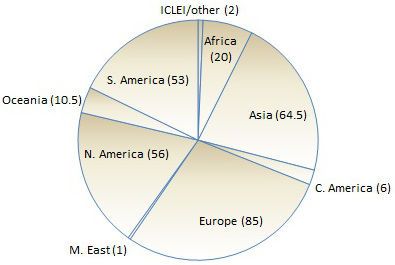
\includegraphics[width=\textwidth]{Fig01.jpg}}
\captionof{figure}{Community gardens in the north of Lisbon (Portugal). \label{Fig01}}
\end{minipage}




\end{multicols}
\vspace{\baselineskip}

\setlength{\tabcolsep}{3pt}
\noindent
\begin{footnotesize}
\begin{minipage}{\columnwidth}\centering
\captionof{table}{Results of a General Linear Model for the proportion of agricultural land under organic farming in French Departments (2008) as a function of plant biodiversity, landscape connectivity, proportion of Natura 2000 protected areas, latitude, longitude, altitude, human population size and department area. The number of data points is 95, the adjusted R$^2$ of the model 0.50, and the intercept 1.457 (s.e. = 2.074).}
\label{Tab01}
\begin{tabular}{lrrrrrrrr}
\toprule
 & N of plant taxa & Landscape connectivity & \% Natura 2000 & Latitude & Longitude & Altitude & Human population & Area \\
\midrule
parameter estimate & 0.264 & 0.047 & 0.113 & -0.084 & 0.003 & 0.038 & 0.056 & 0.327 \\
s.e. & 0.486 & 0.101 & 0.09 & 0.024 & 0.017 & 0.172 & 0.132 & 0.139 \\
\textit{P}-value & 0.59 & 0.64 & 0.21 &\textbf{ \textless0.001} & 0.87 & 0.82 & 0.67 & \textbf{0.02}\\
\bottomrule
\end{tabular}
\end{minipage}

\end{footnotesize}

\vspace{\baselineskip}
\begin{multicols}{2}


\begin{enumerate}[label=\alph*)]
\item
\end{enumerate}